% CHAPITRE 2
% SUIVI VARIABILITE SPATIALE
\singlespacing
\chapter{Sites d'études et méthodologies employées}
\label{ch:ch2}

\minitoc

\newpage
\doublespacing
\section{Présentation de la tourbière de La Guette}

Le site d'étude, la tourbière de La Guette, est l'un des quatre sites du Service National d'Observation des Tourbières (SNOT) qui vise à observer sur le long terme les flux de GES et le bilan de carbone (gazeux, dissout et particulaire) dans des tourbières tempérées notamment vis-à-vis des changements globaux (\url{http://www.sno-tourbieres.cnrs.fr/}).

\begin{figure}[h]
\centering
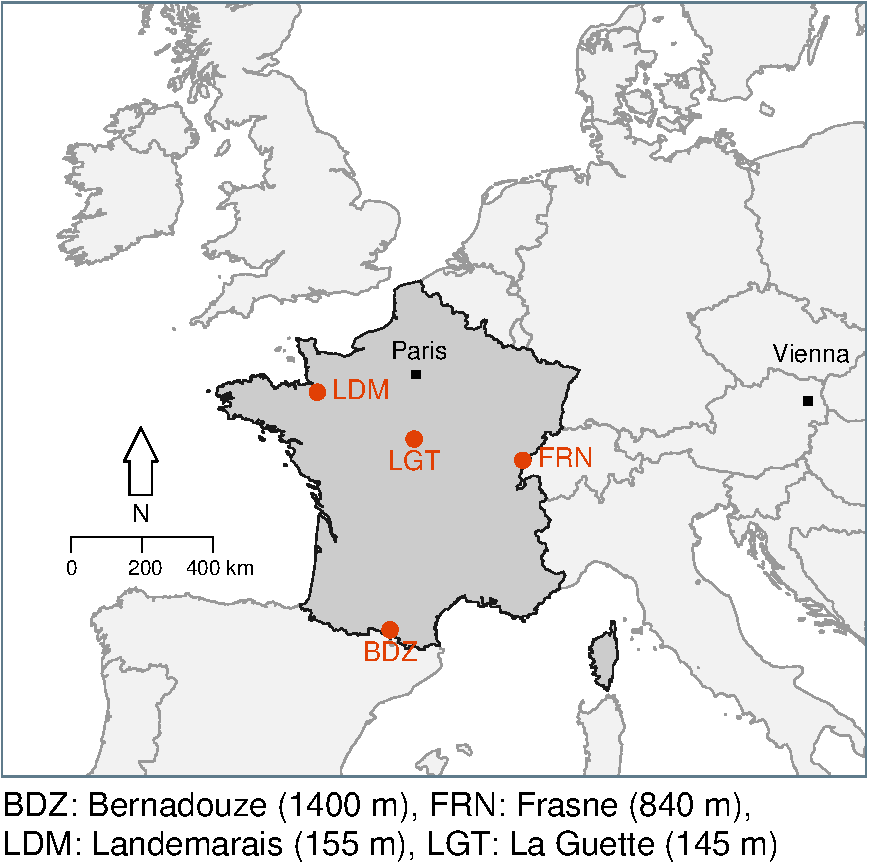
\includegraphics[width=.75\textwidth]{chap2/SNO_siteLocalisation}
\caption{Localisation des sites d'études appartenant au SNOT}
\label{fig:carte_europe}
\end{figure}
%\subsection{La Guette}

La tourbière de La Guette est située à Neuvy-sur-Barangeon, en Sologne (N 47\textdegree19’44”, E 2\textdegree17’04”), dans le département du Cher (Figure~\ref{fig:carte_europe}).
Le site est classé Espace Naturel Sensible par le Conseil départemental du Cher, et également Zone Naturelle d'Intérêt Écologique Faunistique et Floristique (ZNIEFF) et il est intégré au site Natura 2000 « Sologne ».
La tourbière s'étend sur une surface d'une vingtaine d'hectares avec une géométrie relativement allongée (Figure~\ref{fig:carte_LG}).
Cette surface la classe parmi les plus grandes de Sologne (F. Laggoun, communication personnelle).
L'épaisseur moyenne de la tourbe est de \SI{80}{\centi\metre} avec des maximums locaux atteignant \SI{180}{\centi\metre}.
La tourbière de La Guette est probablement topogène, formée par l'accumulation d'eau de pluie dans une cuvette imperméabilisée par une couche d'argile issue d'alluvions de la rivière du même nom (La Guette).
Les précipitations annuelles moyennes sur le site sont de \SI{880}{\milli\metre} et la température moyenne annuelle de \SI{11}{\degreeCelsius} \citep{gogo2011}.
L'eau du site a une conductivité généralement inférieure à \SI{80}{\micro\siemens\per\square\metre} et un pH compris entre 4 et 5.
Ces caractéristiques classent la tourbière parmi les tourbières minérotrophes pauvres en nutriments (\textit{poor fen}).
En collaboration avec le laboratoire de mesure du carbone 14 de Saclay, des datations effectuées sur le site permettent de dire que les premiers dépôts tourbeux datent au moins de \num{4000} ans BP.

Le site a subi un certain nombre de perturbations au cours de son existence.
D'abord la construction avant 1945 d'une route, la D~926, qui coupe l'extrémité sud de la tourbière favorisant son drainage.
Le site a également subi un incendie en 1976.
En 1979 des pins noirs (\textit{Pinus nigra}) sont plantés au nord du site.
Enfin en 2008, le curage du fossé de drainage bordant la route semble entraîner une augmentation significative des pertes d'eau du système.

\begin{figure}
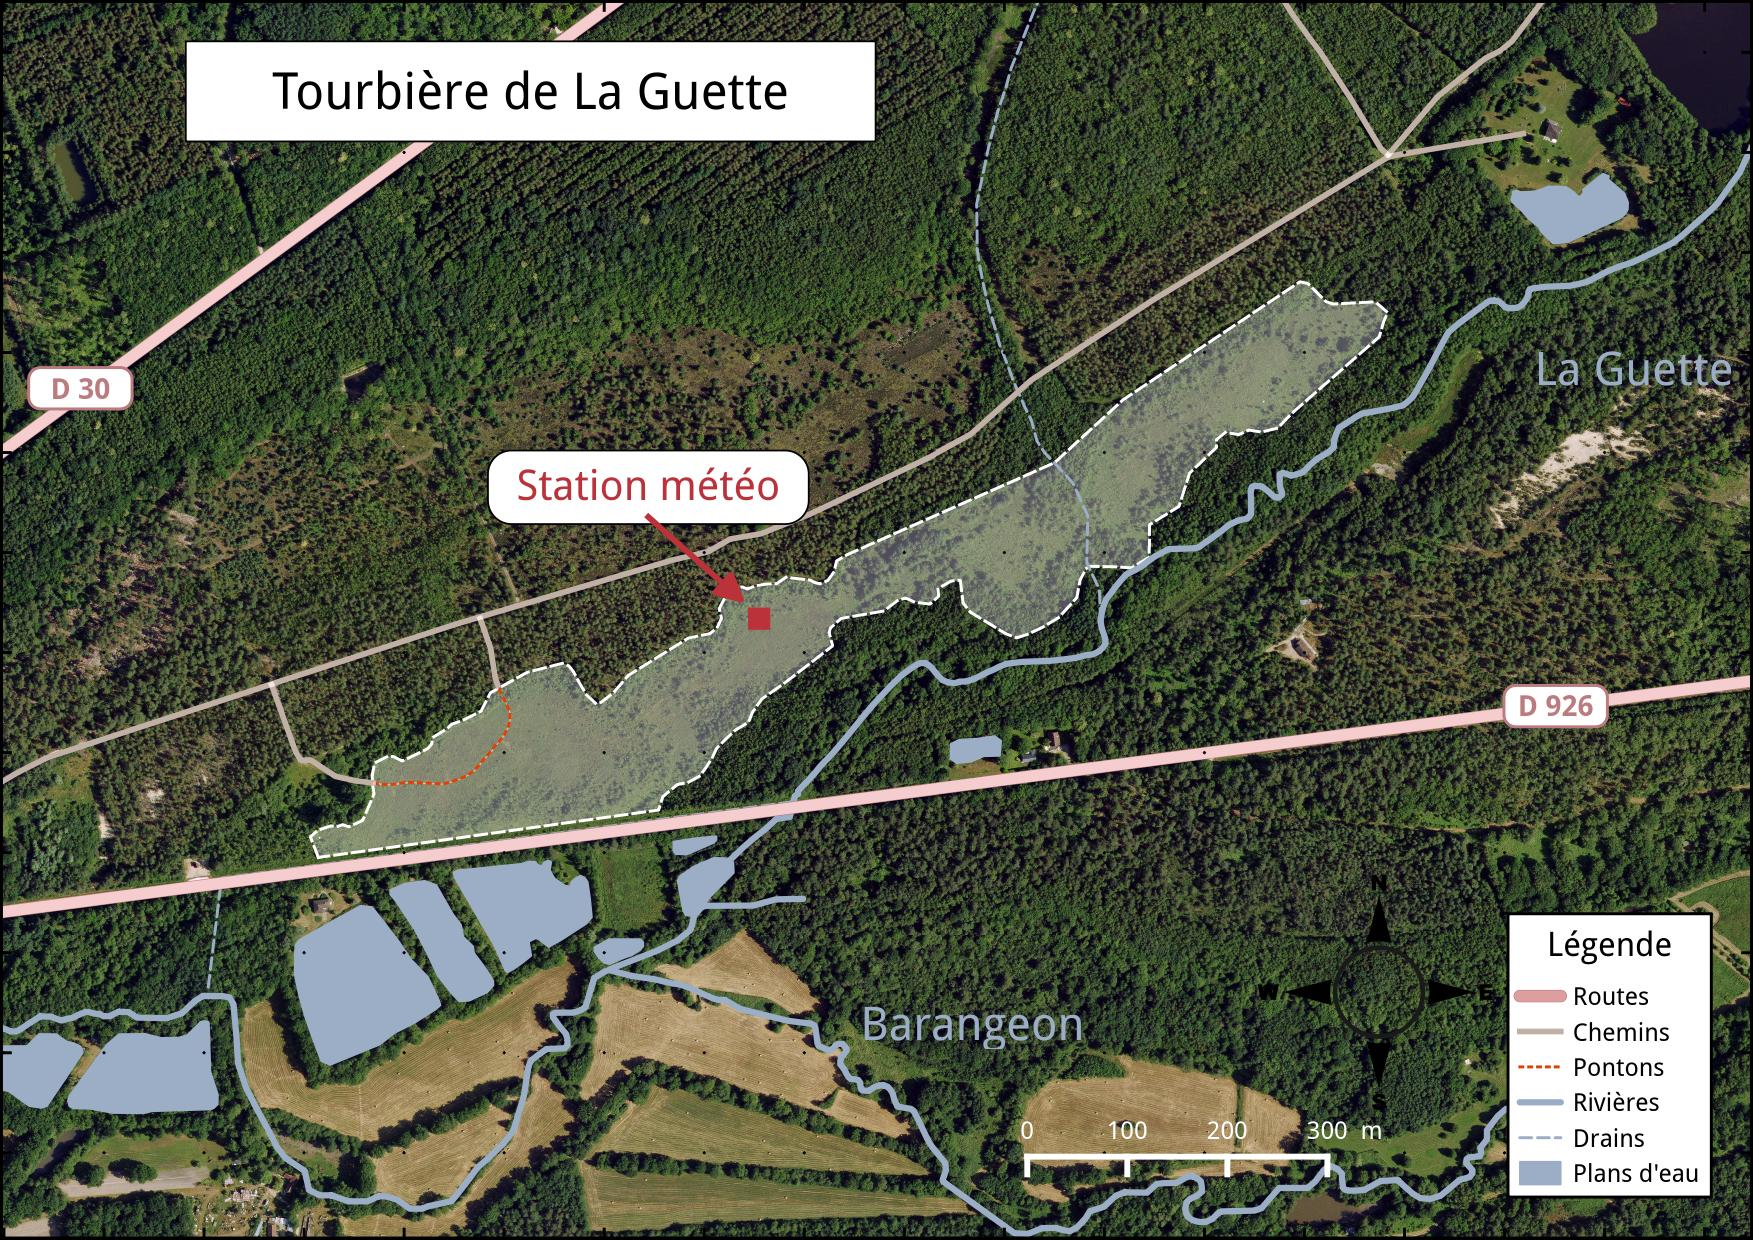
\includegraphics[width=\textwidth]{chap2/carteGL_lowres}
\caption{Carte de la tourbière de La Guette (orthophotographie : BD ORTHO\textsuperscript{\textregistered} -- IGN)}
\label{fig:carte_LG}
\end{figure}

Ces perturbations, ou au moins une partie d'entre elles, ont probablement favorisé l'envahissement du site par une végétation vasculaire, notamment arborée et composée de pins (\textit{Pinus sylvestris}) et de bouleaux (\textit{Betula verrucosa} et \textit{pubescens}).
\citet{viel2015} ont pu calculer, grâce à l'étude de photos aériennes, la vitesse de fermeture du site entre 1945 et 2010, estimée à \SI{2020}{\square\metre\per\year} avant l'incendie de 1976 et à \SI{3469}{\square\metre\per\year} après.
La tourbière est également envahie de façon importante par la molinie bleue (\textit{Molinia caerula}) de la famille des \textit{Poaceae} (Figure~\ref{fig:mol}), leur présence favorisant la dégradation des matières organiques \citep{gogo2011}.
Sont également présentes sur le site un certain nombre d'espèces caractéristiques des tourbières comme les sphaignes, principalement \textit{Sphagnum cuspidatum} et \textit{Sphagnum rubellum}, qui forment des tapis (Photo~\ref{fig:sphg_erio}).
%Un tapis de sphaignes en cours de formation est visible sur la photo~\ref{fig:sphg_erio}.
Des Linaigrettes à feuilles étroites (\textit{Eriophorum augustifolium}), une plante de la famille des \textit{Cyperaceae} caractéristique des marais et des landes tourbeuses sont également visibles sur la tourbière \citep{rameau2008}.
Des bruyères sont également présentes de façon importante sur le site avec notamment \textit{Erica tetralix}, parfois appelée la Bruyère des marais, de la famille des \textit{Ericaceae} (Figure~\ref{fig:erica}).
De la même famille est présente sur le site, mais de façon moindre, la Callune (\textit{Calluna vulgaris}).
L'ensemble de ces espèces tendent à préférer les milieux riches en matières organiques et pauvres en nutriments \citep{rameau2008}.
D'autres espèces sont présentes sur ce site, notamment \textit{Rhynchospora alba} de la famille des \textit{Cyperaceae}, \textit{Juncus bulbosus} de la famille de \textit{Juncaceae}, et des Droséras, une plante insectivore de la famille des \textit{Droseraceae} (Annexe~\ref{sec:photos_veg}, Figure~\ref{fig:dro}) . 

\begin{figure}[htbp]
    \centering
    \begin{subfigure}[b]{.98\textwidth} % "0.45" donne ici la largeur de l'image
        \centering 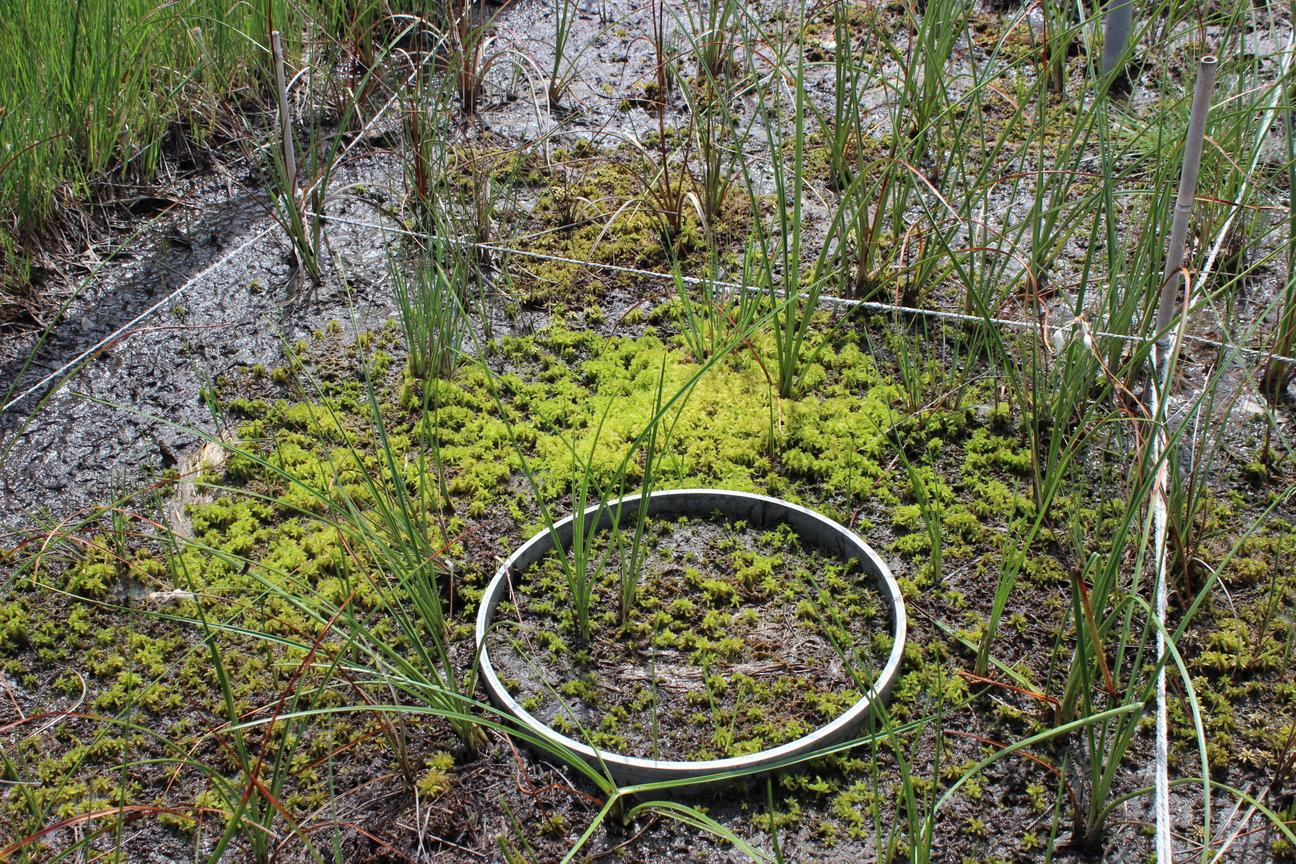
\includegraphics[trim=5cm 0cm 0cm 10cm, clip=true, width=\textwidth]{chap2/sphaigne_eriophorum_c.jpg}
        \caption{\textit{Sphagnum} -- \textit{Eriophorum augustifolium}}\label{fig:sphg_erio}
    \end{subfigure}
    
%    ~ % ce symbole ajoute un espacement horisontal entre les premières deux images
    \begin{subfigure}[b]{0.49\textwidth}
%        \centering 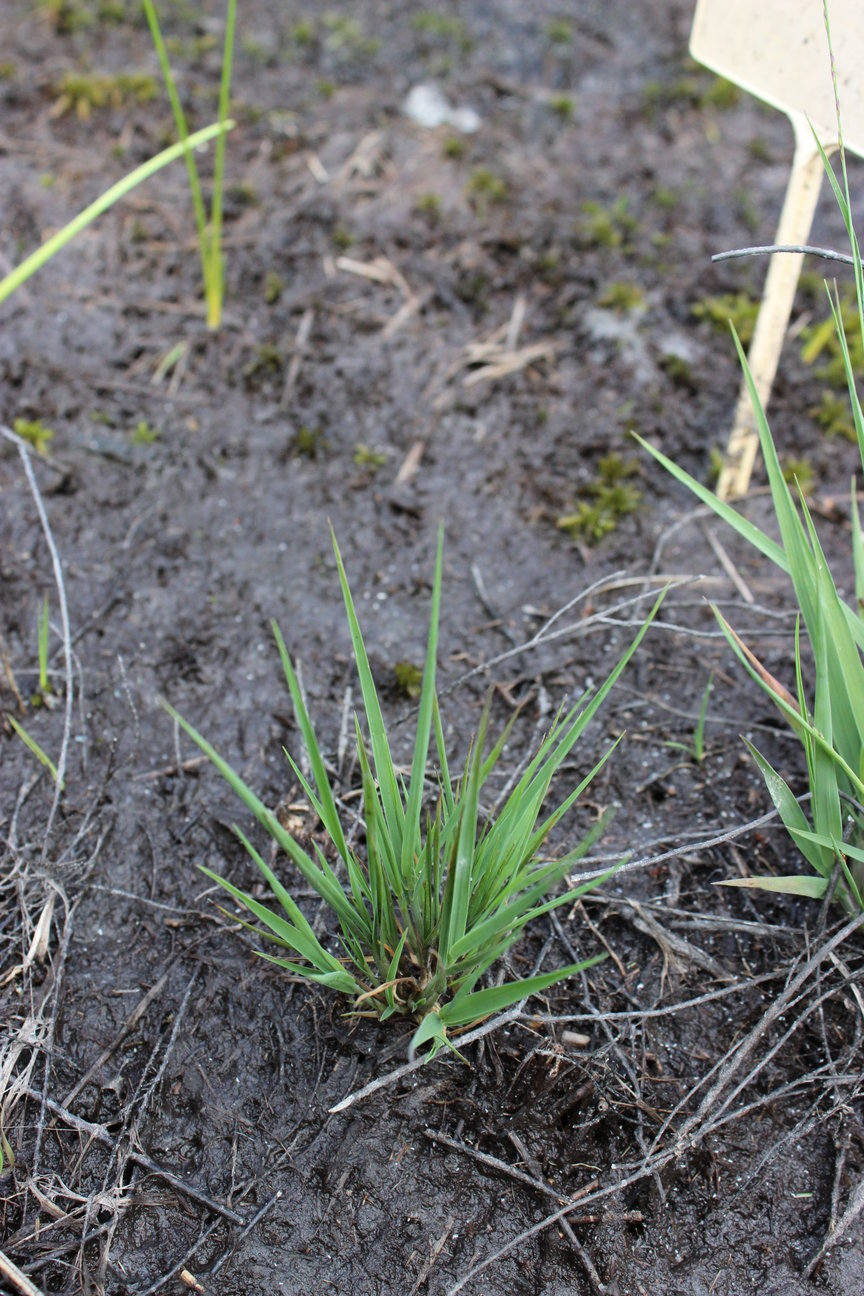
\includegraphics[trim=0cm 0cm 0cm 0cm, clip=true, width=\textwidth]{chap2/molinia_caerulea_c.jpg}
        \centering 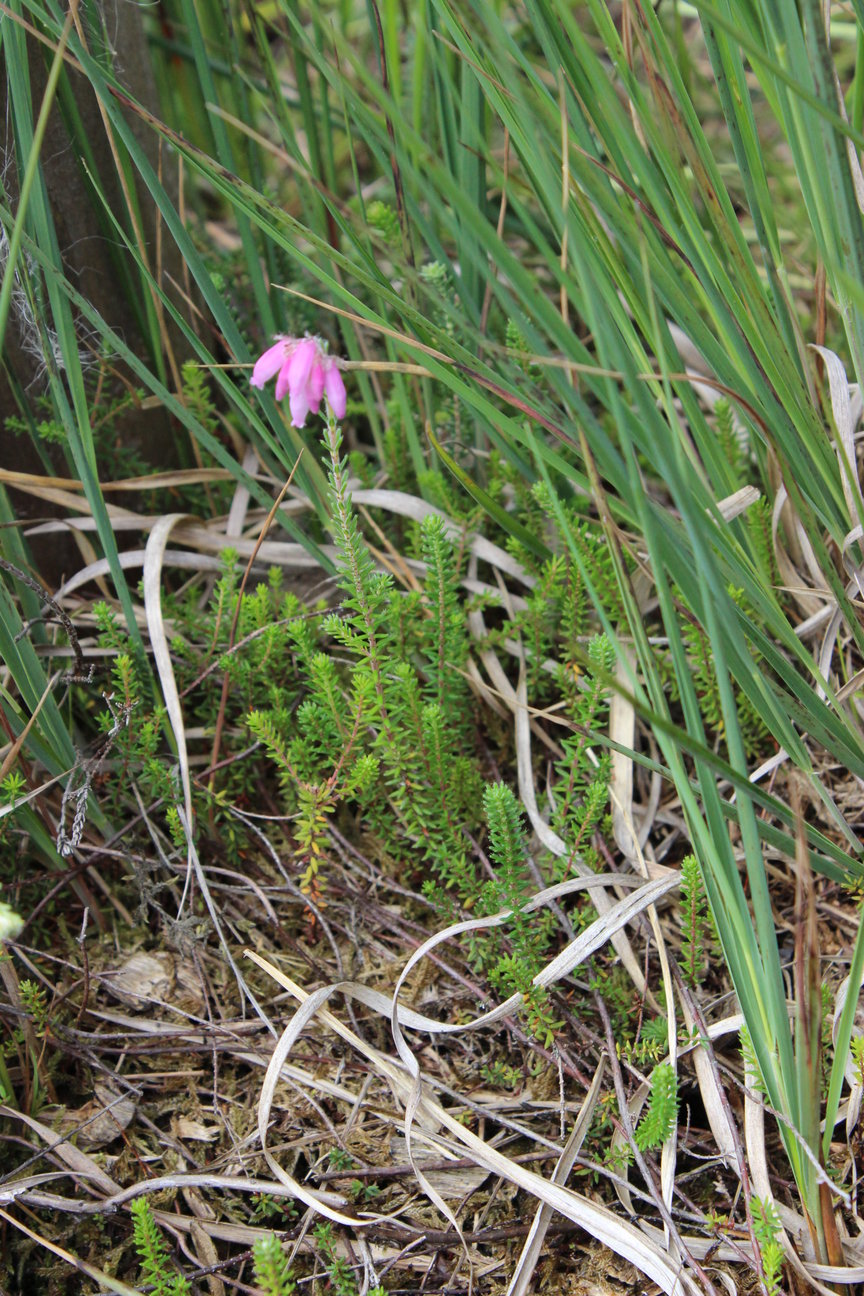
\includegraphics[trim=0cm 4cm 0cm 0cm, clip=true, width=\textwidth]{chap2/erica_tetralix_c.jpg}
        \caption{\textit{Erica tetralix} -- \textit{Molinia caerulea}}\label{fig:erica}
    \end{subfigure}
    % la ligne blanche correspond au retour à la ligne après le deuxième image
    \begin{subfigure}[b]{0.49\textwidth}
        \centering 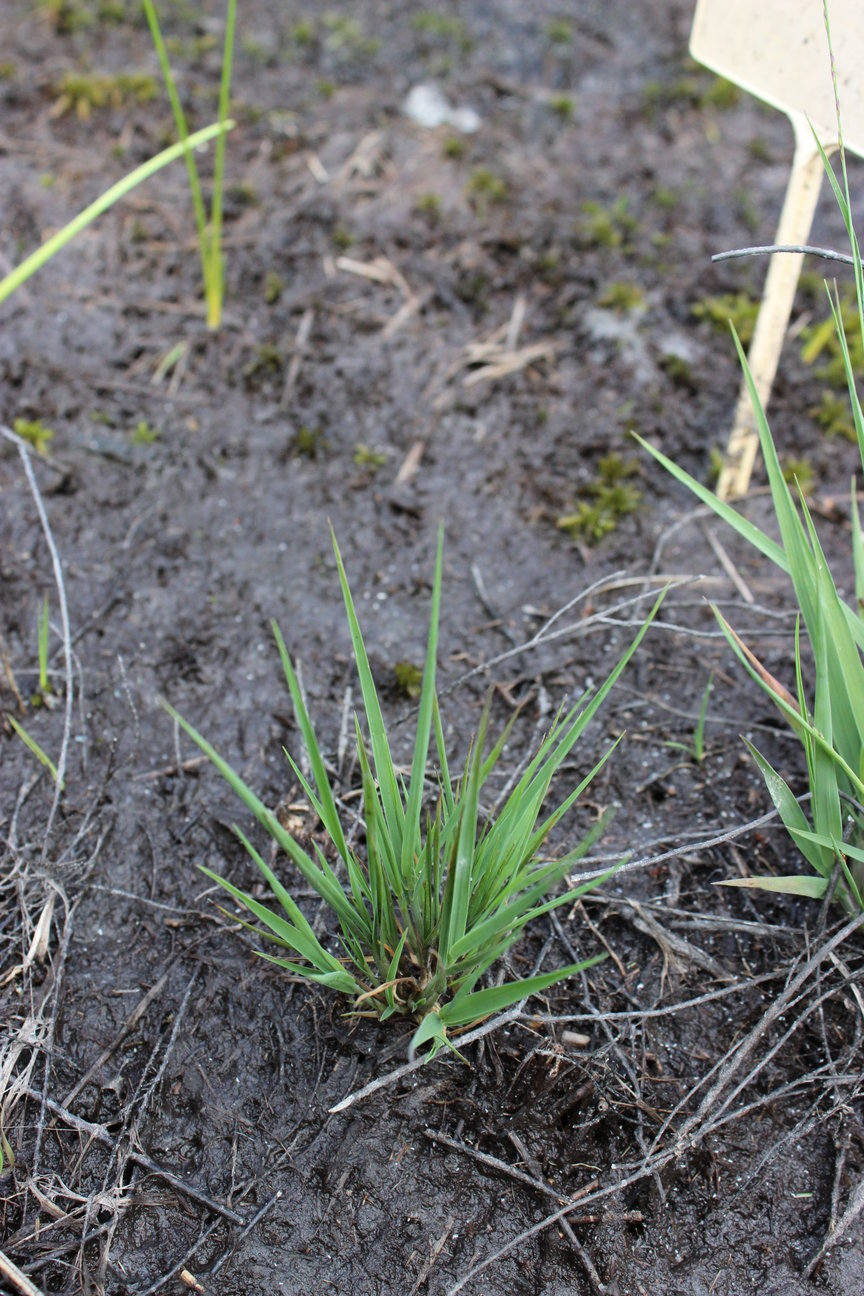
\includegraphics[trim=0cm 2cm 0cm 2cm, clip=true, width=\textwidth]{chap2/molinia_caerulea_c.jpg}
%        \centering 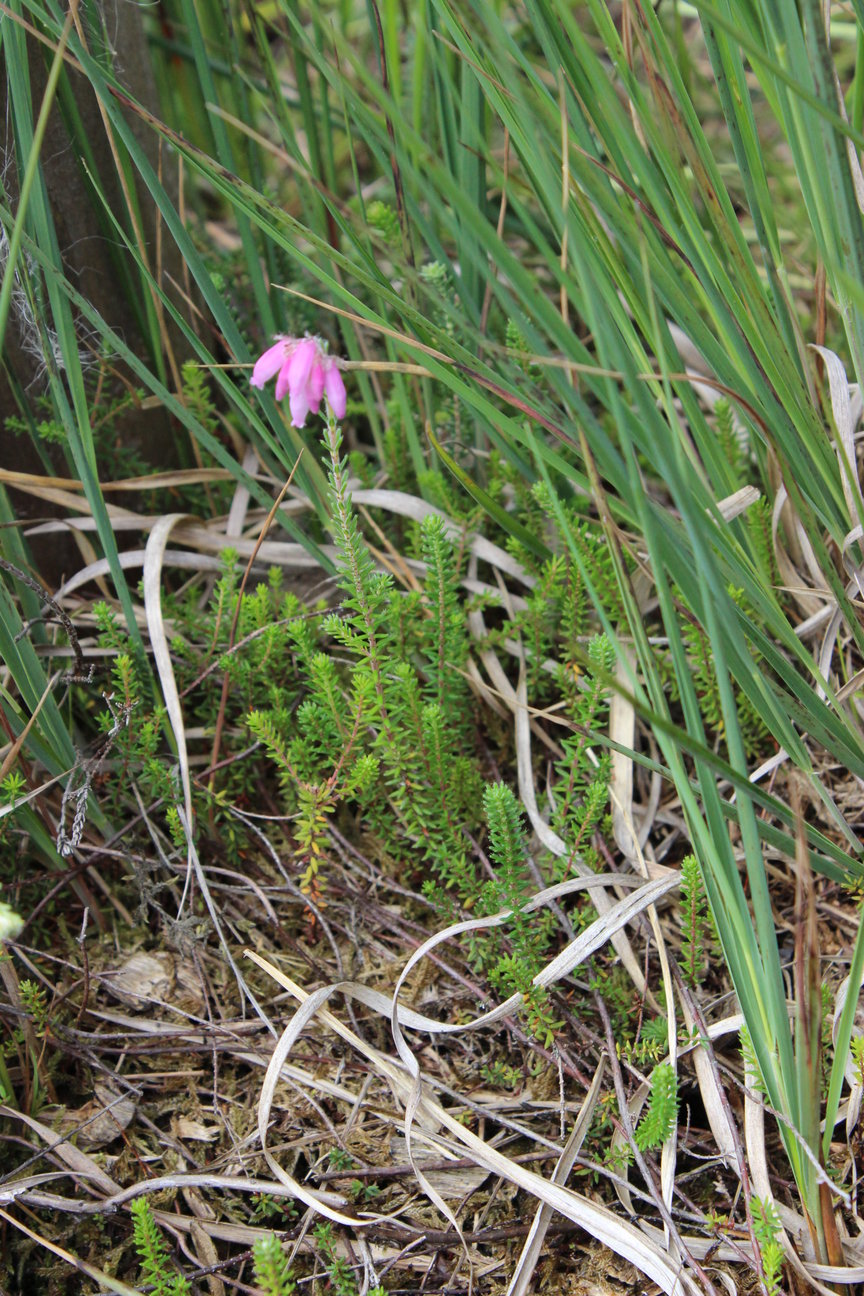
\includegraphics[trim=0cm 0cm 0cm 0cm, clip=true, width=\textwidth]{chap2/erica_tetralix_c.jpg}
        \caption{\textit{Molinia caerulea}}\label{fig:mol}
    \end{subfigure}
%    ~

%    \begin{subfigure}[b]{.8\textwidth}
%        \centering 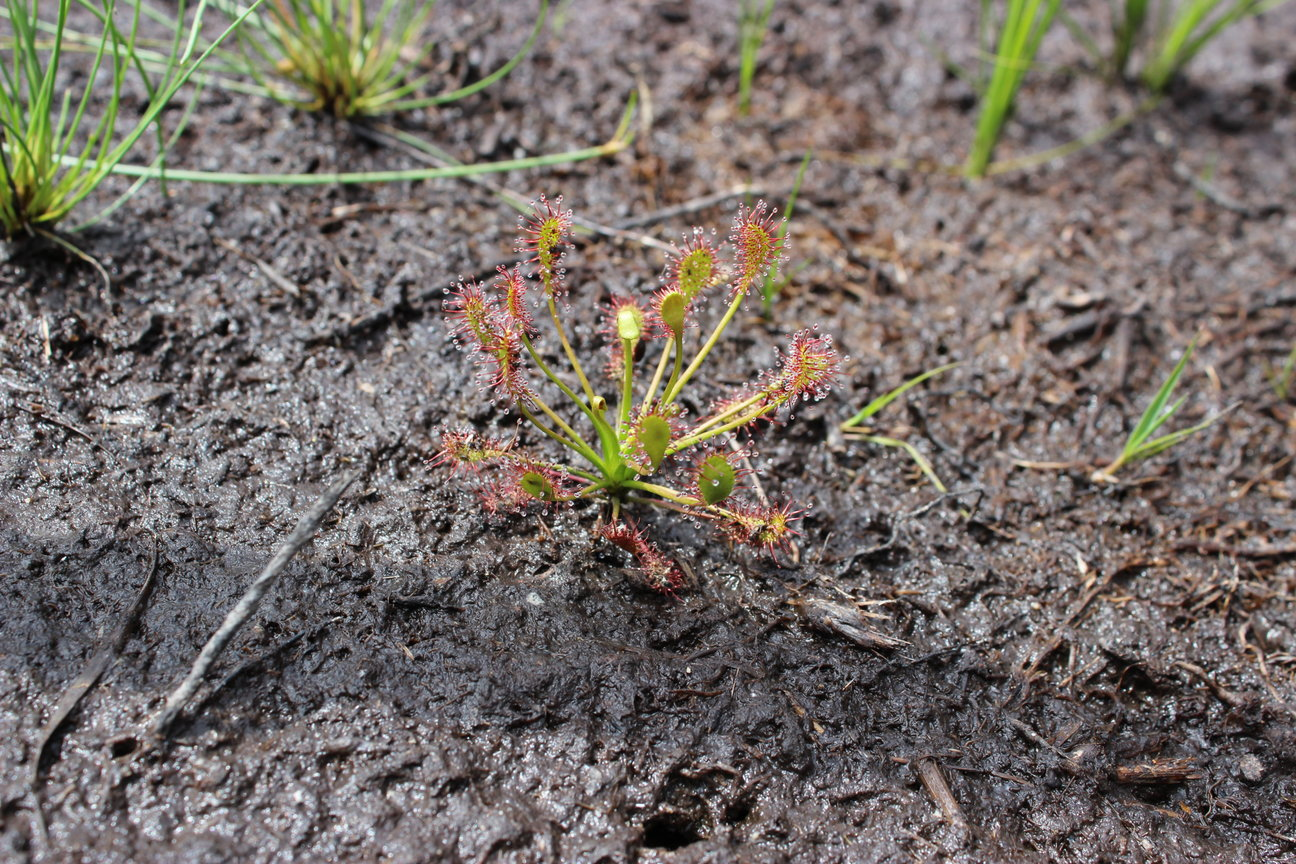
\includegraphics[trim=2.5cm 5cm 2.5cm 5cm, clip=true, width=\textwidth]{chap2/drosera_c.jpg}
%        \caption{drosera}\label{fig:dro}
%    \end{subfigure}
    \caption{Végétation présente sur le site de La Guette et suivie lors des campagnes de mesures.}\label{fig:veg}
\end{figure}


%\begin{figure}
%\centering
%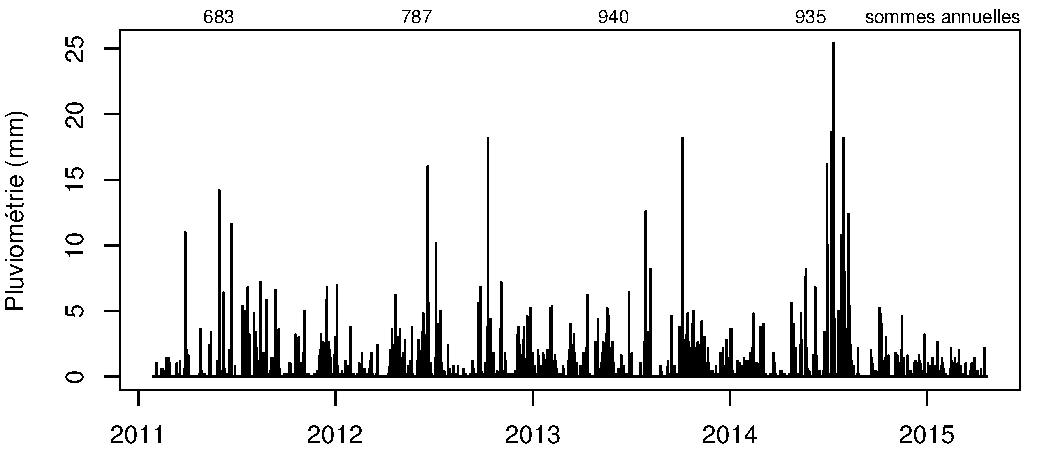
\includegraphics[width=\textwidth]{chap2/pluvio}
%\caption{Évolution du niveau de la pluviométrie, en \si{\mm}, des années 2011 à 2014}
%\label{fig:pluvio}
%\end{figure}
%
%\begin{figure}
%\centering
%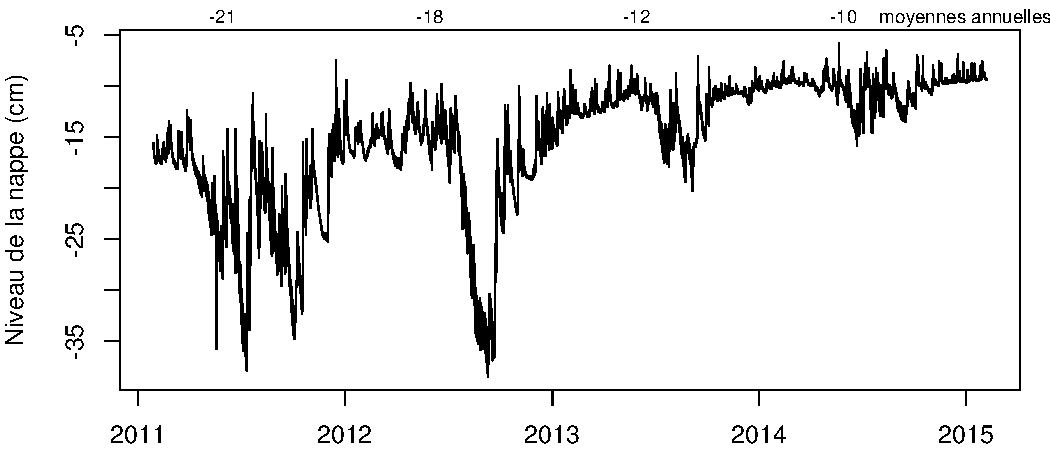
\includegraphics[width=\textwidth]{chap2/WTL}
%\caption{Évolution du niveau de la nappe, en cm par rapport à la surface, des années 2011 à 2014}
%\label{fig:WTL}
%\end{figure}
%
%\begin{figure}
%\centering
%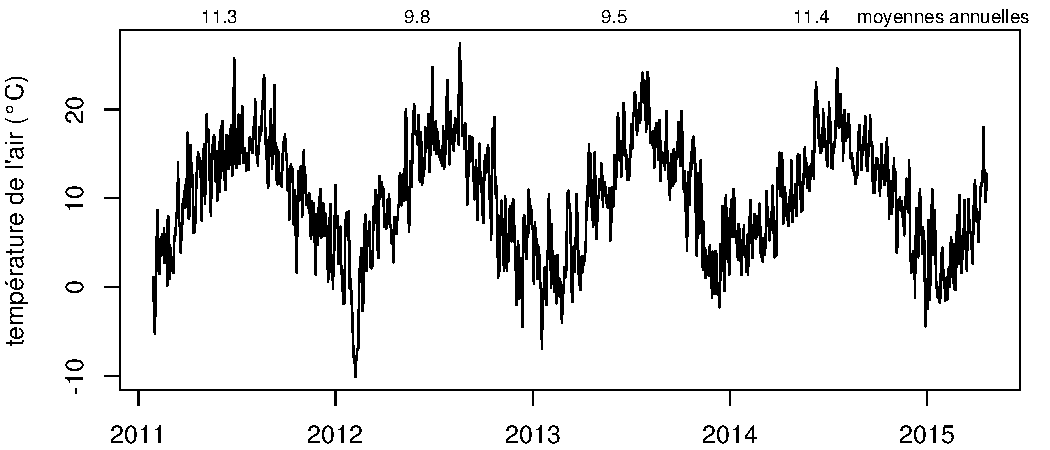
\includegraphics[width=\textwidth]{chap2/tair}
%\caption{Évolution de la température de l'air (en \textdegree C) des années 2011 à 2014}
%\label{fig:tair}
%\end{figure}

\begin{figure}
\centering
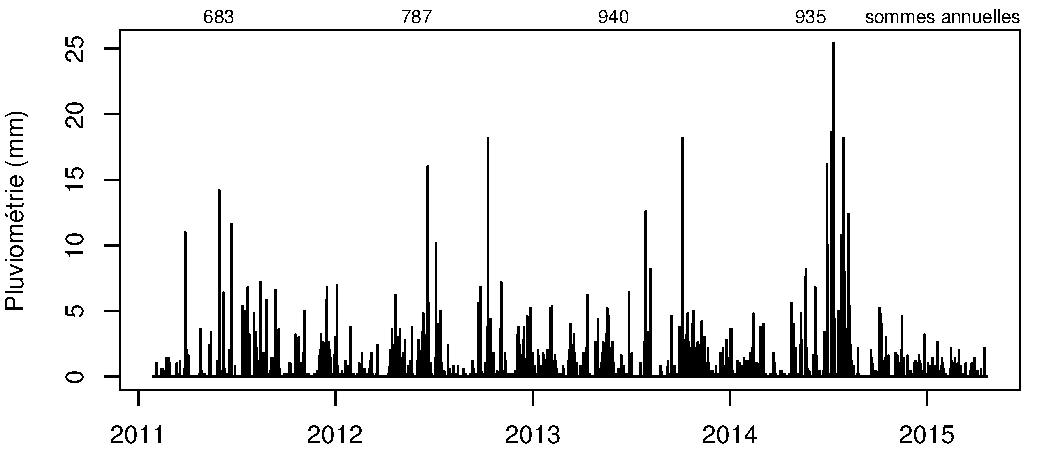
\includegraphics[width=\textwidth,center]{chap2/pluvio}\\
\caption{Évolution du niveau de la pluviométrie, en \si{\mm}, des années 2011 à 2014}
\label{fig:pluvio}
%\vfill
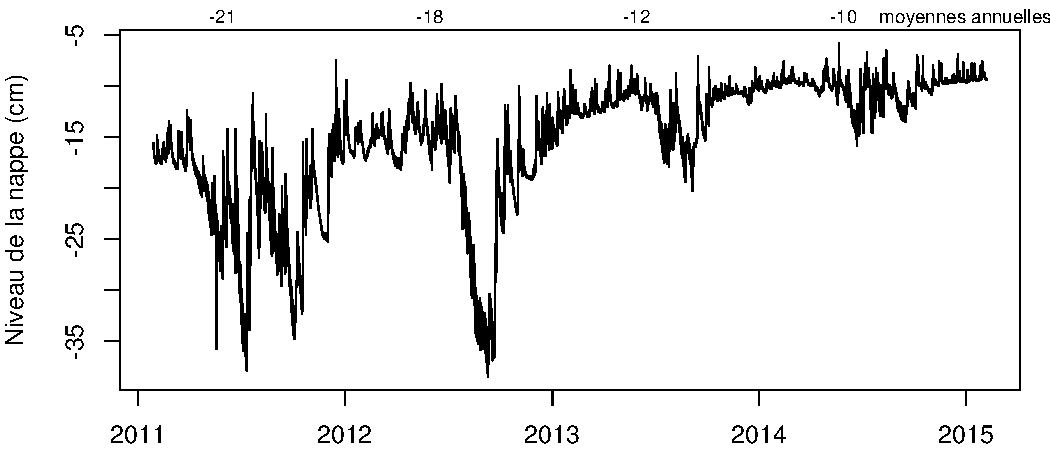
\includegraphics[width=\textwidth, center]{chap2/WTL}\\
\caption{Évolution du niveau de la nappe, en cm par rapport à la surface, des années 2011 à 2014}
\label{fig:WTL}
%\vfill
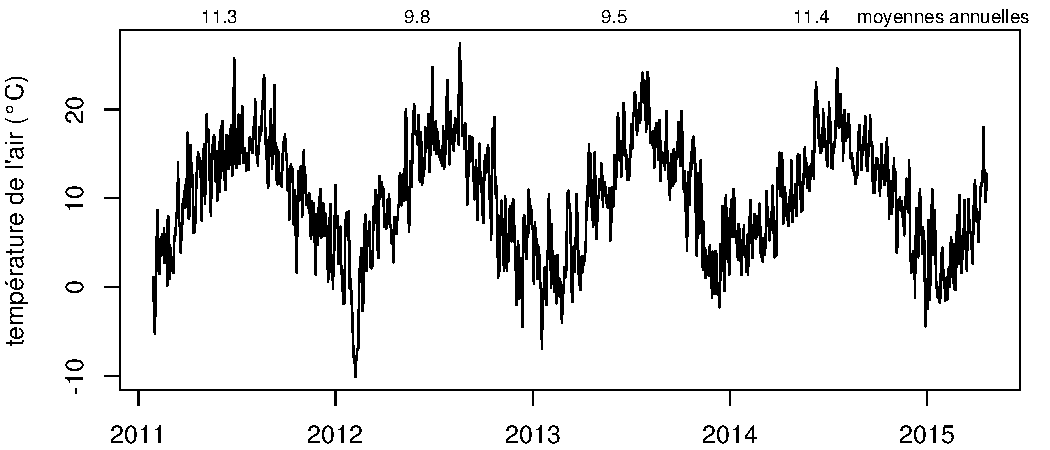
\includegraphics[width=\textwidth,center]{chap2/tair}
\caption{Évolution de la température de l'air (en \textdegree C) des années 2011 à 2014}
\label{fig:tair}
\end{figure}

%Au cours des dernières années,
Le suivi météorologique et hydrologique effectué dans le site depuis 2010 montre que les précipitations sont relativement différentes avec deux années plus sèches que la moyenne avant 2013 et deux années plus humides en 2013 et 2014 (Figure~\ref{fig:pluvio}).
On observe également cette dualité vis-à-vis du niveau de la nappe.
Avant 2013, les étés sont marqués par des étiages importants avec des baisses du niveau de nappe allant jusqu'à \SI{-60}{\cm} en 2012 (Figure~\ref{fig:WTL}).
Après 2013, les étiages sont beaucoup moins importants sur le site (Figure~\ref{fig:tair}).
Les variations inter-annuelles de la température moyenne de l'air semblent moins marquées.
L'année 2011 est très proche de 2014 avec une température moyenne supérieure à \SI{11}{\degreeCelsius}.
De la même façon, les années 2012 et 2013 sont très proches avec des températures moyennes inférieures à  \SI{10}{\degreeCelsius}.


\singlespacing
\section{Autres sites du service national d'observation}
\doublespacing

Bien que moins étudiés, les autres sites du SNOT, Bernadouze, Frasne et Landemarais ont également fait l'objet d'un suivi ponctuel en 2013.
La tourbière de Bernadouze de \SI{3.75}{\hectare} de surface, est située à \SI{1400}{\metre} d'altitude dans les Pyrénées, en Ariège (N 42\textdegree 48’09”, E 1\textdegree25’24”).
%Elle est relativement petite avec \SI{3.75}{\hectare} seulement.
La tourbière de Frasne est située à \SI{840}{\metre} d'altitude dans le Doubs (N 46\textdegree49’35”, E 6\textdegree10’20”) et s'étend sur une surface de \SI{98}{\hectare} (partie active).
Enfin, la tourbière de Landemarais est située en Ille-et-villaine (N 48\textdegree26’30”, E 1\textdegree10’54”) à \SI{154}{\metre} d'altitude et s'étend sur \SI{23}{\hectare}.
Les températures annuelles moyennes de ces trois sites sont respectivement de 6, 7,5 et \SI{11}{\degreeCelsius} et les précipitations annuelles de \num{1700}, \num{1400} et \SI{870}{\milli\meter}.

Au sein du SNOT et à travers les différentes expérimentations et observations réalisées sur les sites, de nombreuses mesures ont été effectuées : des mesures de \coo et de \chh ainsi que d'un certain nombre de facteurs contrôlant.
%La méthodologie utilisée pour les mesurer étant transverse aux différentes expérimentations elle sera détaillée dans ce chapitre.
Les méthodologies utilisées de façon transverse aux différentes expérimentations sont décrites ci-après, celles plus spécifiques le seront dans le chapitre qui les concerne.

\section{Mesures de flux de gaz}
\label{sec:clsd_chbr_method}

\subsection{Présentation des méthodologies principales}

%\subsubsection{Méthode de mesure des flux de gaz}

Différentes techniques existent pour estimer les flux de gaz nécessaires au calcul des bilans de carbone.
Les méthodes les plus utilisées sont les techniques de chambres et les techniques micro-météorologiques.
%D'autres méthodes, moins souvent utilisées, existent comme l'utilisation du ratio C:N (Kirk2015)

De façon générale, les méthodes de chambres consistent à placer une enceinte (ou chambre) sur une zone de l'écosystème dont on souhaite mesurer les flux.
Ces chambres peuvent être ouvertes : la mesure se fait lorsque le gaz à l'intérieur de la chambre est à l'équilibre avec celui à l'extérieur, ou fermées : le gaz à l'intérieur de la chambre n'est pas à l'équilibre avec celui à l'extérieur.
Elles peuvent également être dynamiques, lorsqu'un système de pompe permettant notamment de transporter le gaz jusqu'à l'analyseur est présent, ou statique si le système est sans flux artificiel.
Trois grandes techniques de chambres existent : d'abord les chambres \textbf{dynamiques ouvertes} qui se basent sur un état d'équilibre et mesurent une différence de concentration d'un gaz dont une partie passe par la chambre et l'autre non. 
Cette méthode nécessite un système de pompe et donc l'existence d'un flux.
Ensuite les chambres \textbf{dynamiques fermées} qui mesurent l'évolution de la concentration du gaz au sein de la chambre à l'aide d'un système de pompe permettant l'envoi du gaz dans un analyseur externe mais en utilisant une boucle fermée.
Enfin les chambres \textbf{statiques fermées} qui mesurent également l'évolution de la concentration du gaz au sein de la chambre sans système de pompe.
Dans ce cas soit l'analyseur est présent dans la chambre, soit des prélèvements sont faits à intervalles réguliers puis analysés par la suite en chromatographie gazeuse.

Il faut noter que les dénominations anglaises de ces méthodes doivent faire l'objet d'une attention particulière.
La dénomination \textit{Closed chamber} par exemple est parfois utilisé pour se référer à l'état ou non d'équilibre, comme défini dans ce document, mais parfois également pour désigner les méthodes de chambres sans système de flux ce qui peut prêter à confusion \citep{pumpanen2004}.
Souvent utilisées, les dénominations \textit{open}/\textit{closed} et \textit{dynamic}/\textit{static} sont décrites dans \citet{luo2006161}, une autre convention peut être rencontrée : \textit{flow-through}/\textit{non-flow-through} et \textit{steady state}/\textit{non-steady state} \citep{livingston1995}.

Ces différentes méthodes ont divers avantages et inconvénients : les systèmes sans circulation d'air sont généralement plus faciles à transporter et à utiliser sur le terrain.
L'ensemble des méthodes de chambres fermées ont, par principe, une variation des concentrations en gaz qui, si elle est très importante, peut perturber le gradient de diffusion du gaz.
Malgré tout, ces méthodes sont souvent utilisées car elles ont un coût modeste, et sont très versatiles ce qui permet leur utilisation dans de nombreuses situations.

D'autres méthodes existent comme les méthodes micro-météorologiques, basées sur l'étude des flux turbulents en analysant à haute fréquence la vitesse et la direction du vent.
Ces méthodes sont souvent appelées \textit{Eddy Covariance} ou \textit{Eddy Correlation}.
Elles sont beaucoup plus onéreuses et lourdes à mettre en place mais permettent une acquisition haute fréquence des flux de gaz.
Ces méthodes sont complémentaires aux mesures de chambre, car elles se font sur une zone plus grande que celles mesurées à l'aide de chambres.
La variabilité spatiale est donc intégrée dans la mesure, ce qui peut être un avantage comme un inconvénient.
La grande majorité des bilans pluriannuels sont faits à l'aide de cette méthode.


%\subsection{Présentation des méthodologies possibles}
\subsection{Les mesures de \texorpdfstring{CO\textsubscript{2}}{CO2}}
\label{subsec:ss_mes_co2}

Toutes les mesures de flux de \coo présentées par la suite ont été faites avec les mêmes matériels et le même protocole.
Les chambres utilisées sont en Plexiglas\textsuperscript{\textregistered} et ont été conçues par le LPC2E et fabriquées à l'ISTO.
Ce sont des chambres transparentes, cylindriques, de \SI{30}{\centi\metre} de diamètre pour \SI{30}{\centi\metre} de hauteur.
Les mesures de concentration en \coo à proprement parler ont été faites à l'aide d'une sonde Vaisala CARBOCAP\textsuperscript{\textregistered} GMP~343.
La sonde est directement insérée dans la chambre ainsi qu'une sonde Vaisala HUMICAP\textsuperscript{\textregistered} HMP~75 mesurant l'humidité et la température dans la chambre (Figures~\ref{fig:chb}).

Préalablement aux mesures, des embases sont installées dans le site.
Ce sont des cylindres en PVC d'une hauteur de \SI{15}{\centi\metre} pour \SI{30}{\centi\metre} de diamètre, insérés dans le sol sur 8 à \SI{10}{\centi\metre} de profondeur.
La partie basale et enterrée de ces cylindres a été préalablement percée d'une quarantaine de trous (\SI{1}{\centi\metre} de diamètre) afin de minimiser les impacts de l'embase sur le développement racinaire et permettre les écoulements d'eau.

La méthode mise en œuvre est celle de la chambre statique fermée, aucun système de pompe n'est donc utilisé.
Ceci permet d'avoir un système de mesure relativement léger, facilement transportable et permettant une mise en oeuvre sur l'ensemble du site d'étude.
Une mesure se déroule de la façon suivante :
la chambre est posée sur l'embase, l'analyseur de \coo et la sonde humidité/température sont insérées à l'intérieur.
Un ventilateur de faible puissance est également positionné à l'intérieur de la chambre au préalable afin d'homogénéiser l'air.
1 à \SI{3}{\minute} de stabilisation sont nécessaires après la pose de la chambre afin d'éviter les effets pouvant y être liés, le plus souvent la perturbation d'un gradient de concentration.
L’enregistrement est ensuite lancé.
Les données (concentration en \coo, température, humidité) sont acquises toutes les \SI{5}{\second} pendant \SI{5}{\minute}.
La mesure se déroule donc sur une période de temps relativement courte afin de minimiser les perturbations possibles et d'éviter de s'éloigner des conditions naturelles extérieures.
Dans ce but, les mesures ont parfois été manuellement raccourcies, 2 à \SI{3}{\minute} d'acquisition, si une pente claire se dégageait rapidement, ceci notamment lorsque les conditions météorologiques, chaudes et ensoleillées, laissaient supposer une différence importante vis-à-vis des conditions extérieures.
Deux acquisitions de \coo sont faites à la suite sur une même embase.
La première, avec la chambre transparente nue, permettant l'enregistrement de l'ENE (Figure~\ref{fig:chb}-a).
La seconde avec la chambre recouverte d'une chaussette de tissu occultant, isolant la chambre de la lumière, permettant d'interrompre la photosynthèse et donc d'enregistrer les respirations (RE) (Figure~\ref{fig:chb}-b).

\begin{figure}
	\centering
	\begin{subfigure}[t]{0.5\textwidth}
		\centering
		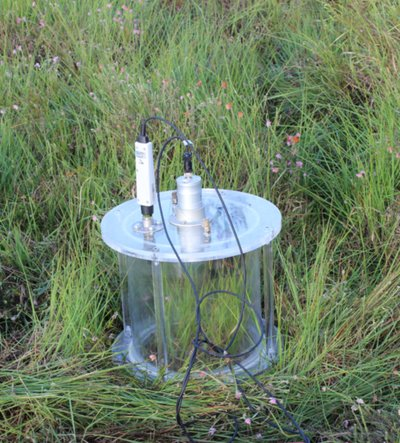
\includegraphics[width=.8\textwidth, frame]{chap2/chb_ENE}
	\end{subfigure}%
	\begin{subfigure}[t]{0.5\textwidth}
		\centering
		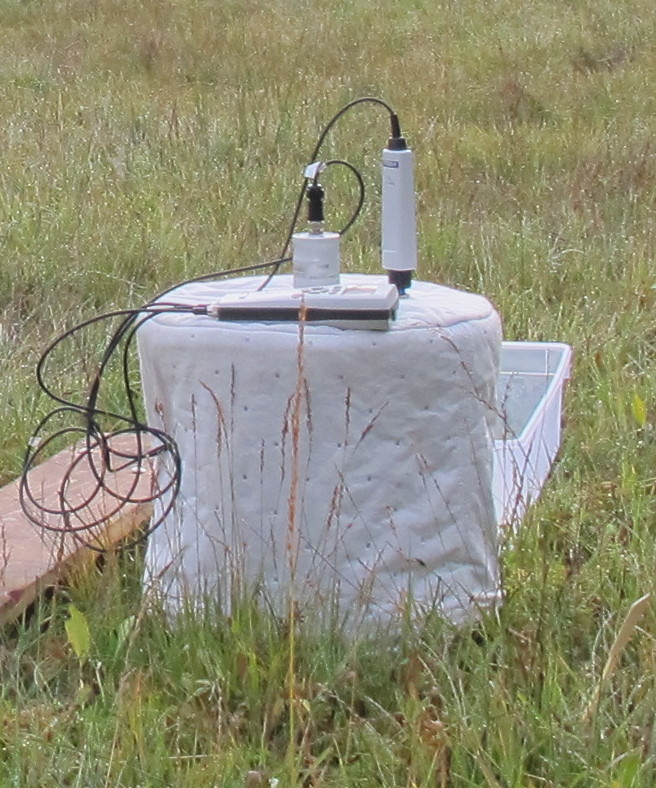
\includegraphics[width=.8\textwidth, frame]{chap2/chb_ER}
	\end{subfigure}%

	\begin{subfigure}[t]{0.5\textwidth}
		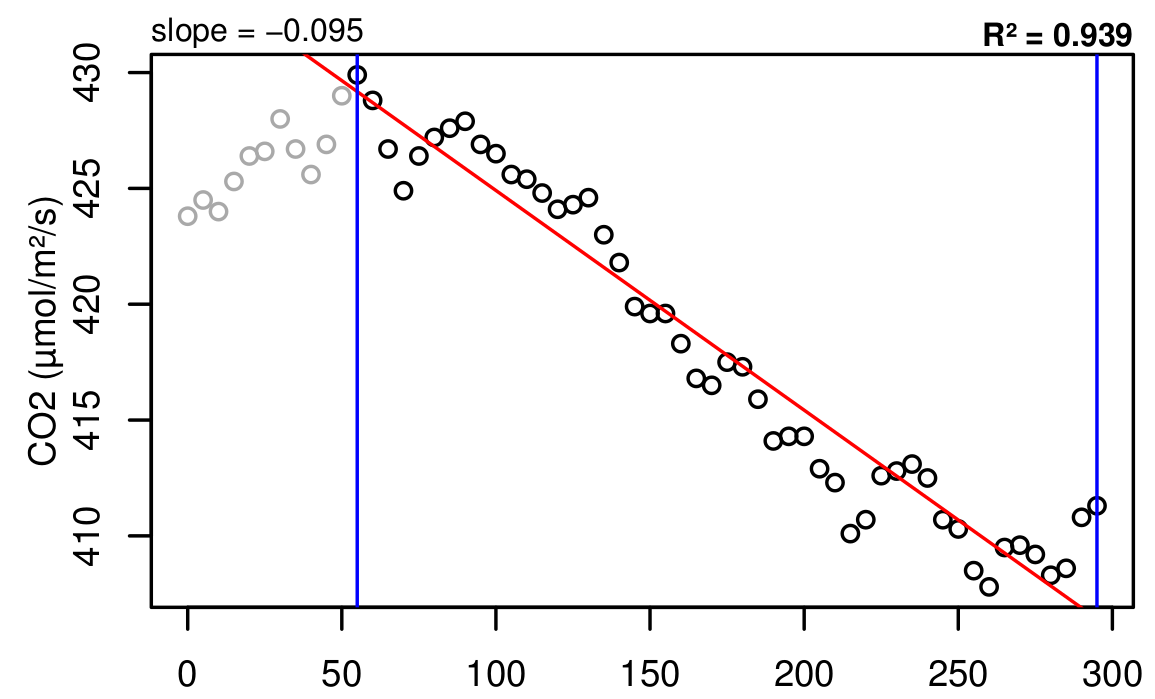
\includegraphics[width=\textwidth]{chap2/chb_ENE_reg}
		\caption{Mesure de l'échange net de l'écosystème}
	\end{subfigure}%
	\begin{subfigure}[t]{0.5\textwidth}
		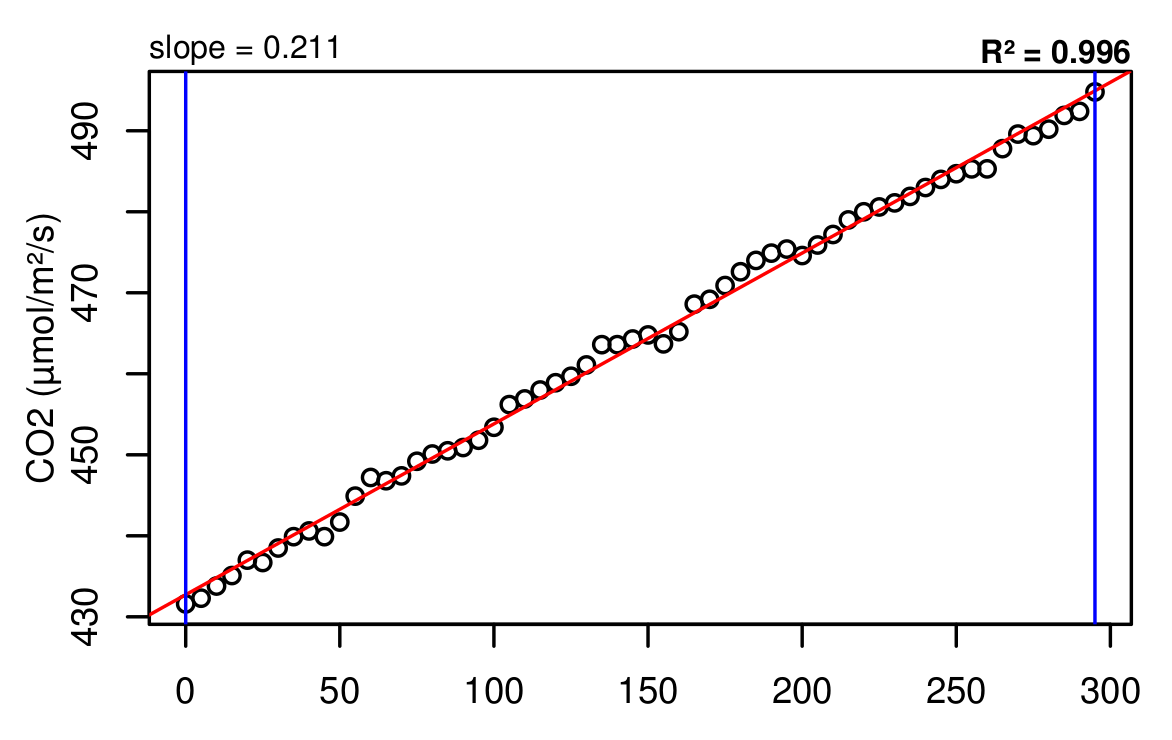
\includegraphics[width=\textwidth]{chap2/chb_ER_reg}
		\caption{Mesure de la respiration de l'écosystème}
	\end{subfigure}
%    \caption{Caption place holder}
\caption{Mesures de \coo et partitionnement des flux}
\label{fig:chb}
\end{figure}


De nombreux écueils peuvent rendre une mesure inexploitable. D'abord le placement de la chambre : cela peut sembler trivial mais positionner la chambre au milieu d'herbacées et de bruyères n'est pas toujours évident. 
Plus anecdotiquement, des sphaignes gelées recouvrant les bords de l'embase rendent la pose de la chambre difficile voire impossible. 
Enfin selon l'heure de la journée, des gradients de concentration peuvent être présents et augmenter localement les concentrations de \coo de façon importante allant jusqu'à saturer la sonde.

Au vu du volume de données acquises et souhaitant garder l'intérêt de mesures manuelles, à savoir le contrôle humain des flux et des conditions de mesure, j'ai développé un outil de traitement facilitant le contrôle et le calcul des flux.
Ceci afin d'éviter de recourir à des seuils arbitraires (typiquement une valeur de R$^{2}$) pour le contrôle de la qualité des données, mais également de permettre une reproductibilité et un traçage des modifications effectuées sur les données brutes.
Ce travail est présenté dans l'annexe~\ref{sec:pckg_m70r}.

\subsection{Les mesures de \texorpdfstring{\chh}{CH4}}

\begin{figure}
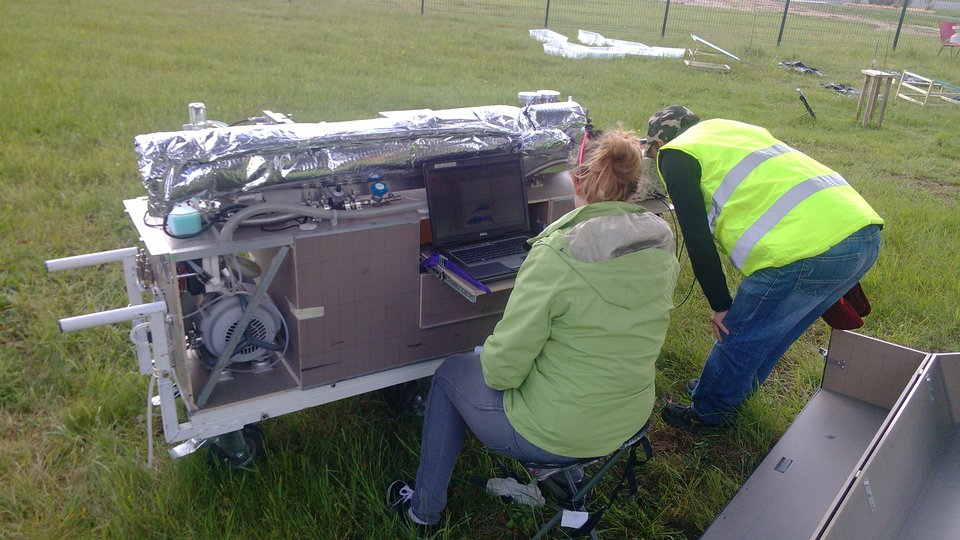
\includegraphics[width=\textwidth]{chap2/SPIRIT_terrain}
\caption{SPIRIT}
\label{fig:SPIRIT}
\end{figure}

Les mesures de \chh ont été réalisées avec une chambre aux caractéristiques similaires à celles utilisées pour les mesures de \coo à l'exception de l'interface avec l'analyseur.
En effet la taille de ce dernier ne permettait pas de l'insérer directement dans la chambre comme l'analyseur de \coo.
La méthode de la chambre dynamique fermée a été utilisée pour réaliser ces mesures.
Elle diffère donc légèrement de celle utilisée pour le \coo puisqu'elle nécessite la mise en oeuvre d'un système de pompe pour transporter le gaz jusqu'à l'analyseur.
%Les mesures de concentration en \chh ont été réalisée à l'aide du SPIRIT 
L'instrument utilisé pour analyser la concentration en \chh est le SPIRIT (SPectromètre Infra Rouge In-situ Troposphérique) (Figure~\ref{fig:SPIRIT}).

Le SPIRIT est un spectromètre infra-rouge développé par le LPC2E.
La spectrométrie infra-rouge se base sur la mesure de l'absorption d'un rayonnement infrarouge par des molécules.
%Pour une molécule, cette absorption est variable selon les longueurs d'ondes permettant de la caractériser, son intensité étant fonction de la concentration (Loi de Beer-Lambert).
Les longueurs d'ondes absorbées par une molécule lui sont spécifiques et permettent de la caractériser, de plus l'intensité de cette absorption est fonction de sa concentration  (Loi de Beer-Lambert).
%L'absorption est spécifique d'une molécule donnée, les longueurs d'ondes qu'elle absorbe permettent de la caractériser
Cet instrument profite de l'expertise acquise par le laboratoire dans le domaine de la métrologie infra-rouge, notamment avec le développement de son ancêtre le SPIRALE (SPectroscopie Infra Rouge par Absoption de Lasers Embarqués).
Plus petit et plus léger (\SI{100}{\kilo\gram}), le SPIRIT a été développé en différentes versions, en fonction des usages.
Il existe actuellement une version sol et une version avion de l'appareil.
Les capacités du SPIRIT sont principalement liées à deux éléments.
Premièrement l'invention d'une cellule à réflexion multiple par le LPC2E \citep{robert2007}, permettant d'adapter facilement la longueur du parcours optique en fonction de la concentration des gaz à mesurer.
Deuxièmement l'utilisation de lasers à cascades quantique (QCL), dont la puissance permet d'augmenter le nombre de réflexion et la sensibilité des mesures d'absorption.
Les QCL installés émettent séquentiellement dans le moyen infra-rouge (\num{2.5} à \SI{25}{\micro\metre}), dans une gamme spécifique aux espèces que l'on souhaite mesurer.
Ce choix est dicté par l'absorbance, à ces longueurs d'ondes, d'un grand nombre d'espèces d'intérêt et l'intensité importante de leurs raies d'absorption.
Après son émission, le laser est divisé en deux : 
la première partie traverse une cellule de référence, contenant un gaz de concentration connue.
La seconde partie traverse une cellule de mesure, contenant le gaz à mesurer.
Les deux parties du laser débouchent finalement sur les détecteurs.
Le spectre d'absorption est divisé par le spectre de référence, ce qui permet de conserver uniquement le signal lié à l'absorption moléculaire. Ce spectre est ensuite comparé à un spectre simulé afin de déterminer les concentrations en gaz.
Le fonctionnement détaillé du SPIRIT-sol est décrit dans \cite{guimbaud2011}.

%C'est un SPectrometre Infra Rouge In-situ Troposphérique (son premier objectif étant d'être emporté lors de campagne avion ou ballon ? pour mesurer le \chh de la troposphère.).
%Il permet la mesure du \chh à haute fréquence.
%Le fonctionnement détaillé de l'appareil est décrit dans \cite{guimbaud2011}.
%\citep{robert2007}

\subsection{Le calcul des flux}

Que ce soit pour le \coo ou le \chh, le flux de gaz est calculé à l'aide de l'équation suivante : 

\begin{equation}
F = \frac{dX}{dt} \times \frac{P}{R \times T} \times \frac{V}{S}
\end{equation}

Avec : 
\begin{itemize}
\item[F :] le flux en \si{\uml}
\item[X :] la concentration en gaz mesuré en \si{\micro\mole\per\mole}
\item[P :] la pression atmosphérique en \si{\kilo\gram\per\metre\per\square\second}
\item[R :] la constante des gaz parfaits en \si{\kilo\gram\square\metre\per\square\second\per\mole\per\kelvin}
\item[T :] la température dans la chambre en \si{\kelvin}
\item[V :] le volume de la chambre en \si{\cubic\metre}
\item[S :] la surface occupée par l'embase en \si{\square\metre}
\end{itemize}

%QUESTIONS :
%
%*Taille des embases ? Effets de bord ?
%*Perturbation du milieu ? (Mesure de végétation, pose de la chambre, mesure pièzo...)
%*Impact de la strate arborée ?
%*Validité des profils de température ?
%Méthode de Chambre fermée (Biais ?)
%
%Améliorations ? (Lister les amélioration à faire ou non)


\section{Facteurs contrôlants}
%Afin de déterminer l'impact de facteurs contrôlants sur ces flux, mesurer les flux ne suffit pas il faut également mesurer les variables environnementales dont on pense qu'elles seront des facteurs contrôlants important.
En plus des mesures de flux de gaz, des variables environnementales ont été parallèlement mesurées.
La description des techniques et matériels communs aux différentes expérimentations utilisées est développée ci-dessous.
Cependant leur mise en œuvre ou caractéristiques spécifiques, comme la fréquence des mesures, sera décrite individuellement au niveau des parties détaillant chacune des expérimentations.

\subsection{Acquisitions automatisées}

Un certain nombre de variables environnementales ont été acquises automatiquement à l'aide d'une station d'acquisition Campbell\textsuperscript{\textregistered}.
Cette station a été installée au centre de la tourbière de La Guette en 2010 (Figure~\ref{fig:carte_LG}).
%Les paramètres météorologiques ont été mesurés, en un point, au centre de la tourbière (Figure~\ref{fig:carte_LG})(\textbf{carte ?}) à l'aide d'une station d'acquisition Campbell installée sur le site en 2008.
Jusqu'au 20 février 2014 l'acquisition des variables s'est effectuée à une fréquence horaire.
Depuis cette date la fréquence d'acquisition a été augmentée à une demie heure.
Les paramètres enregistrés sont la pression atmosphérique, l'humidité relative de l'air, la pluviosité, l'irradiation solaire, la vitesse et la direction du vent. 
%(\textbf{détail du matos ?}).
Cette même station a également permis l'acquisition de la température de l'air et de la tourbe à \num{-5}, \num{-10}, \num{-20} et \SIlist{-40}{\cm}.
Installées à la même époque, quatre sondes de mesure du niveau de la nappe d'eau permettent le suivi du niveau de la nappe dans la tourbière.

\subsection{Acquisitions manuelles}

Les variables acquises manuellement, spécifiques à chaque expérimentation, seront détaillées dans leur chapitre respectif.
% sont la température de l'air et la pression atmosphérique à l'aide d'un XXX, la température de la tourbe (XXXX), l'humidité du sol (XXX), le PAR, le niveau de la nappe (avec un mètre ruban), des hauteurs de végatation (mètre ruban)
% la recouvrement de végétation réalisé à l'oeil (à la louche),

%\subsection{Protocole d'estimation de la végétation}


%\begin{figure}
%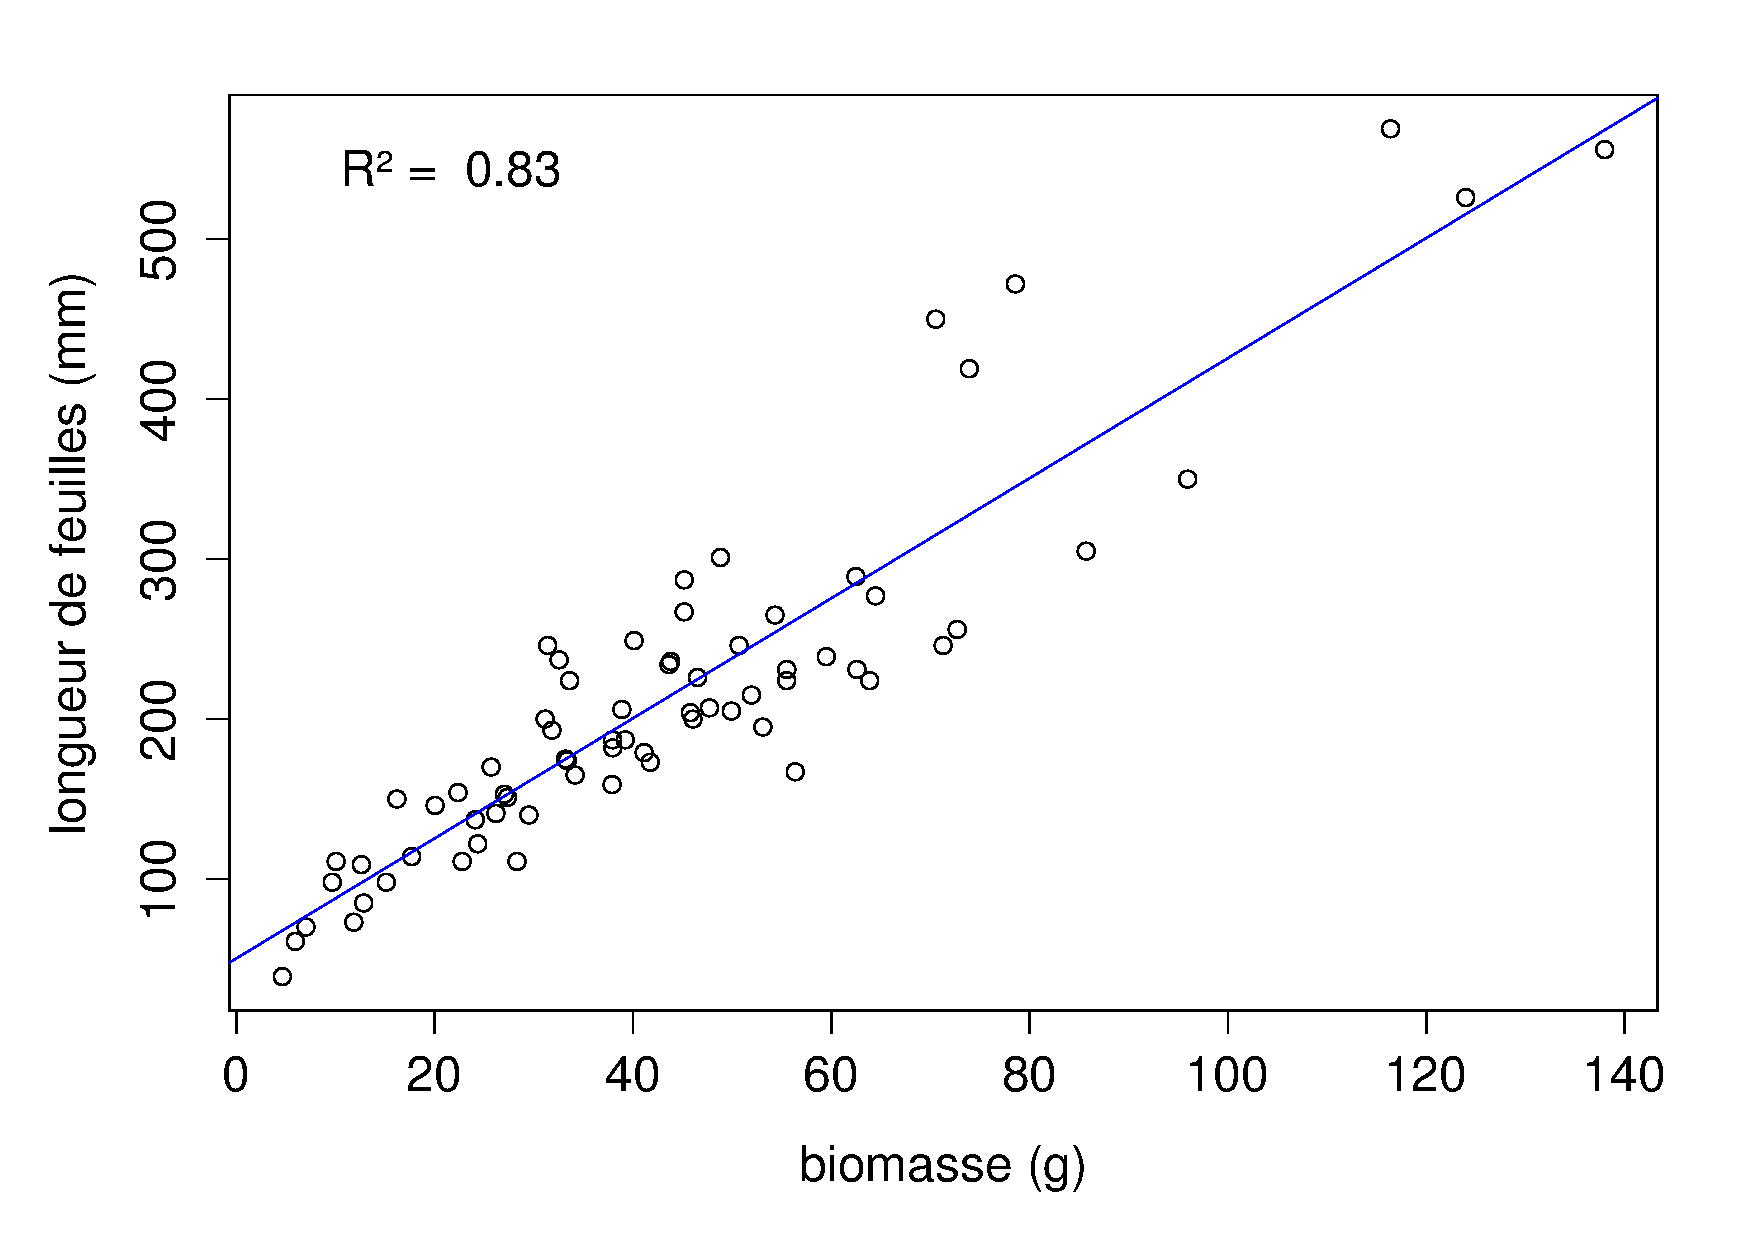
\includegraphics[width=.5\textwidth]{chap2/mol_lon_bioM}
%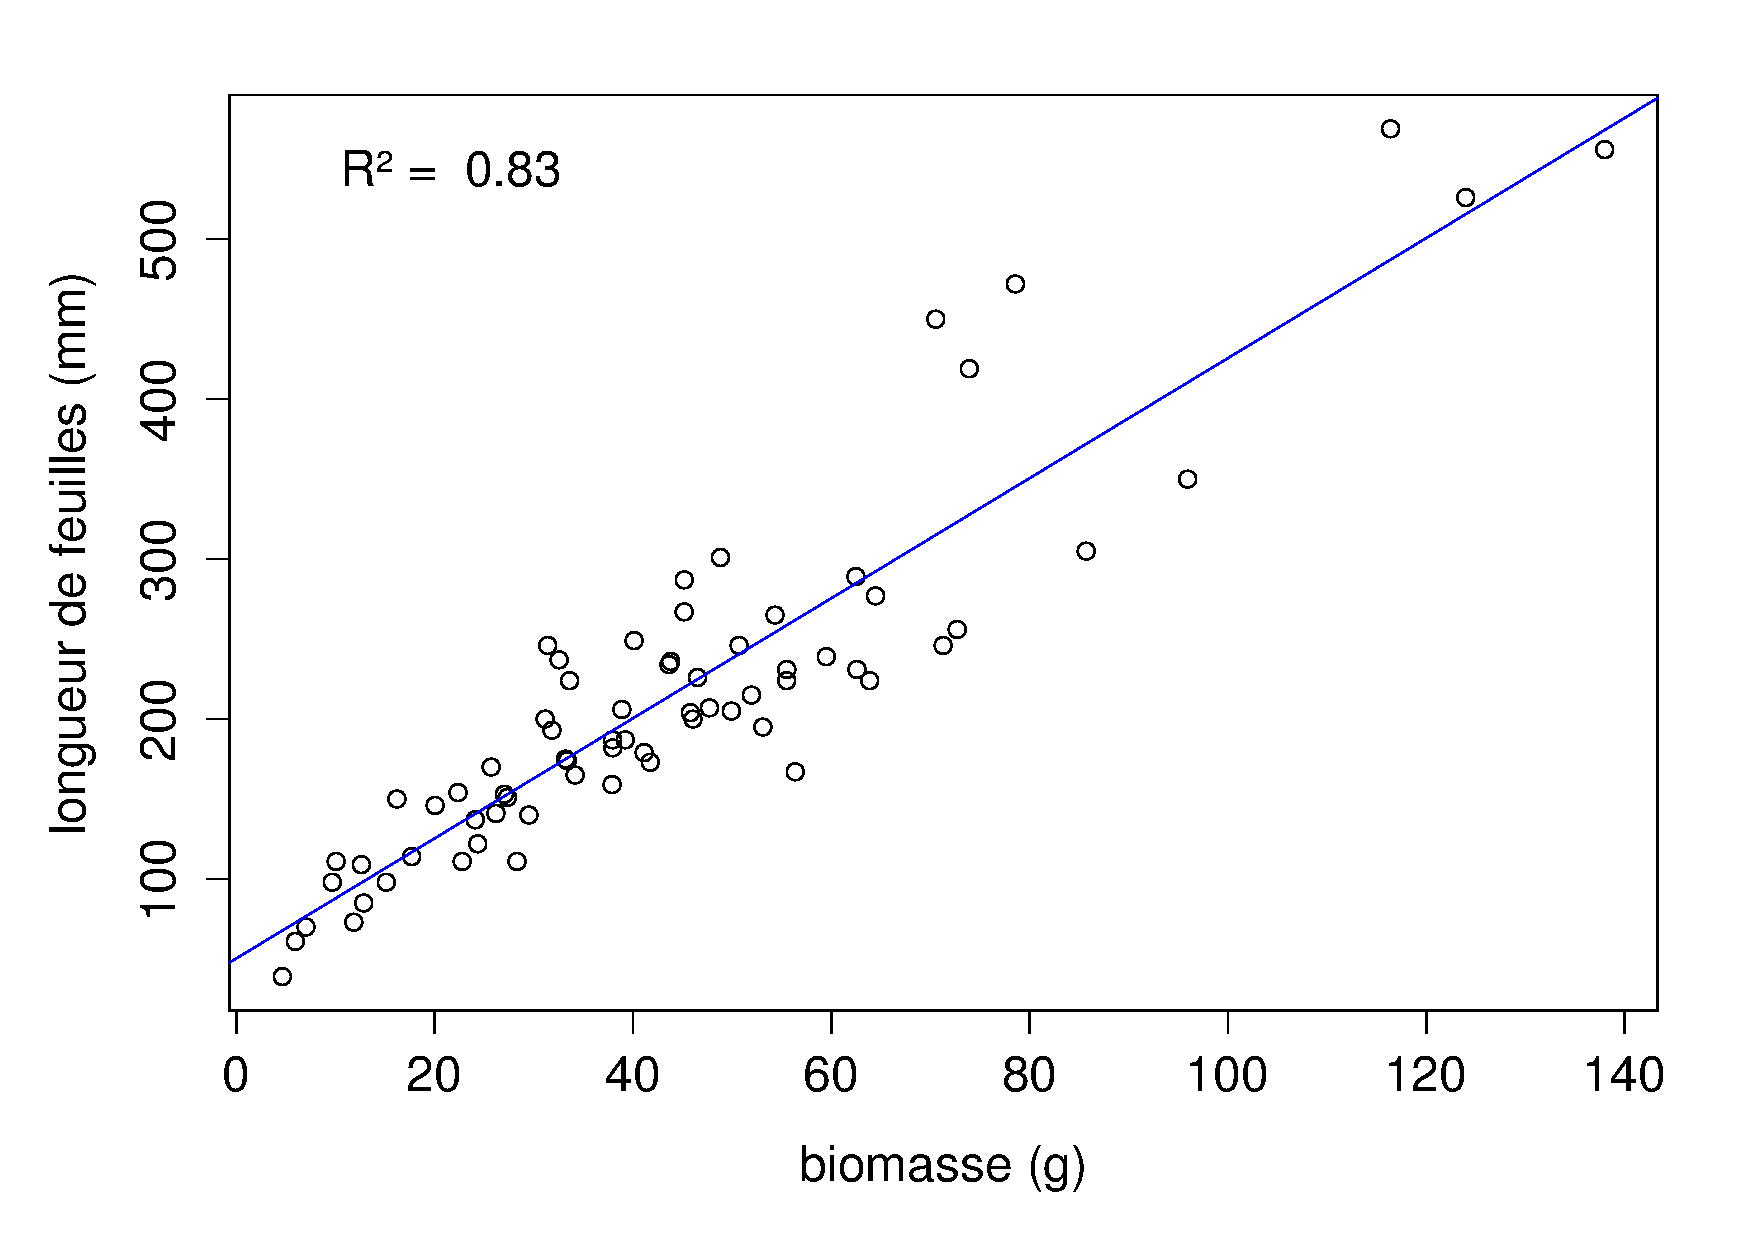
\includegraphics[width=.5\textwidth]{chap2/mol_lon_bioM}
%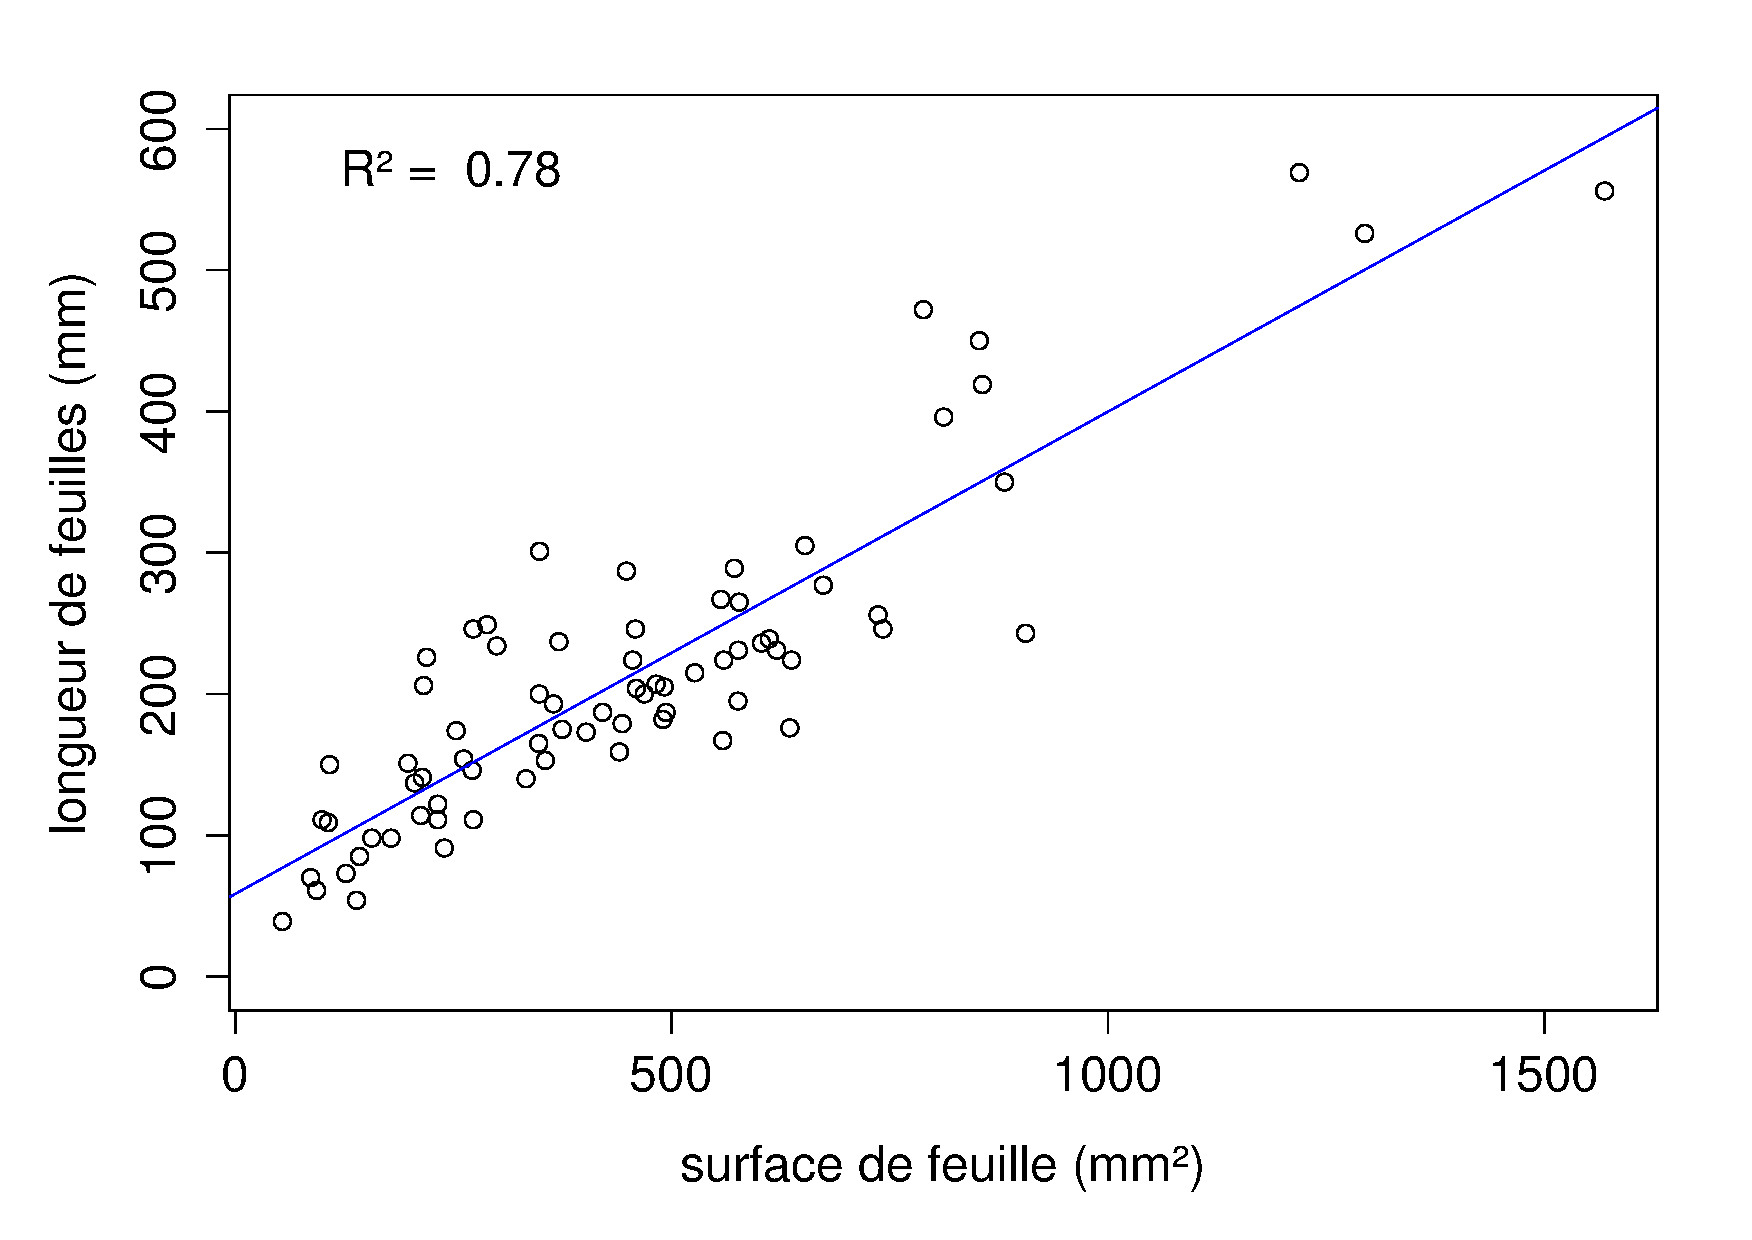
\includegraphics[width=.5\textwidth]{chap2/mol_lon_surf}
%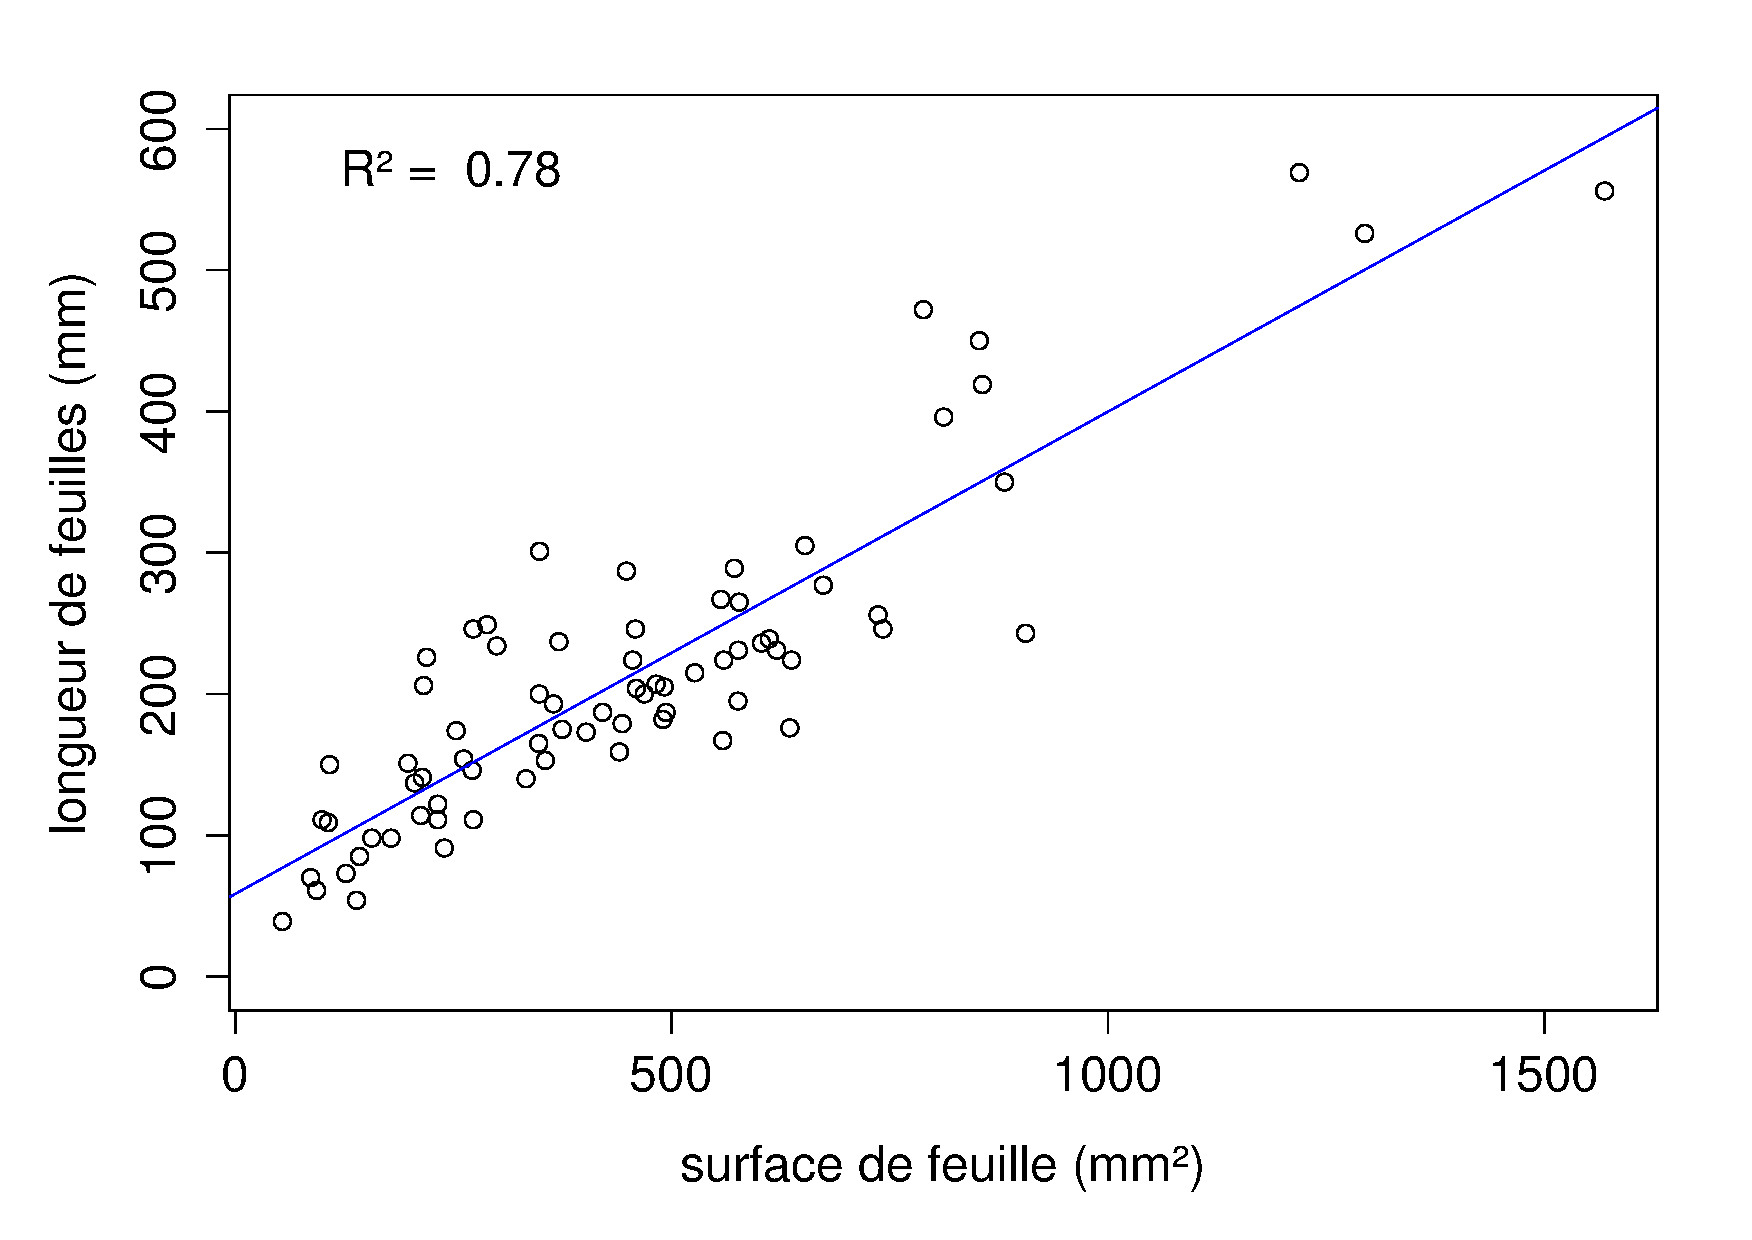
\includegraphics[width=.5\textwidth]{chap2/mol_lon_surf}
%\caption{Calibration de la biomasse herbacées pour \textit{molinia Caerulea} (a), pour \textit{eriophorum} (b) et de la surface de feuille pour \textit{molinia Caerulea} (c), pour \textit{eriophorum} (d) en fonction de la hauteur}
%\label{fig:cal_herb}
%\end{figure}